\subsection{Scenario 1: Stationary grid topology}

\begin{figure}[htb!] 
\center
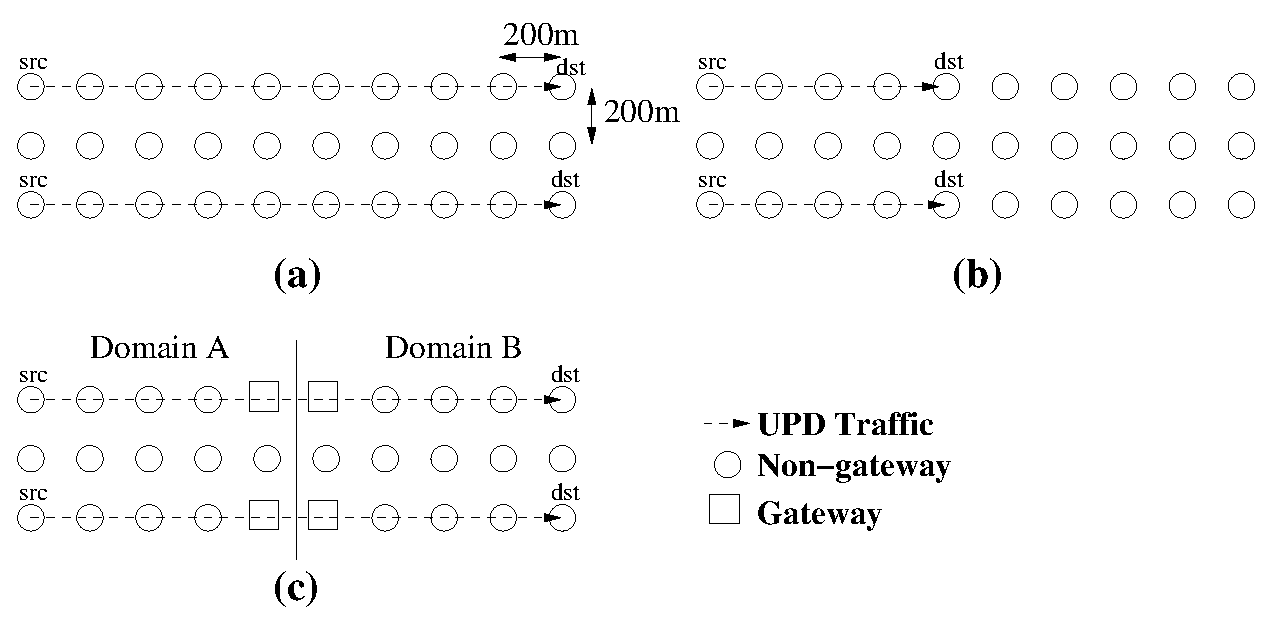
\includegraphics[width=0.47\textwidth]{figs/case1topo.eps}
\caption{Stationary grid topology for: (a) DSDV, and (b) IDRM} 
\label{fig:case1topo}
\end{figure}

We first study the performance of IDRM with
stationary grid topology shown in figure
\ref{fig:case1topo}. 
The goal here is to demostrate the performance of IDRM with multiple domains is
comparable to the performance of the single routing protocol with a signle domain.

We study the performance of IDRM in 3 different settings.
For all 3 cases, there are 2 UDP traffics.
In the first case (figure \ref{fig:case1topo}a), 
the src and the dst of each traffic are separated by 9 hops in a single DSDV domain.
In the second case (figure \ref{fig:case1topo}b), 
the setting is similar to figure \ref{fig:case1topo}a excepts
the src and the dst are separated by 4 hops.
In the last setting (figure \ref{fig:case1topo}c), 
the src and the dst are separated by 9 hops, and they are located in different DSDV domains.

Notice that in figure \ref{fig:case1topo}a and 
figure \ref{fig:case1topo}b, 
all nodes are communicate through one channel, 
while in figure \ref{fig:case1topo}c, 
nodes are using 3 independent channels 
(one for domain A, one for IDRM, and one for domain B). 

\begin{figure}[htb!] 
\center
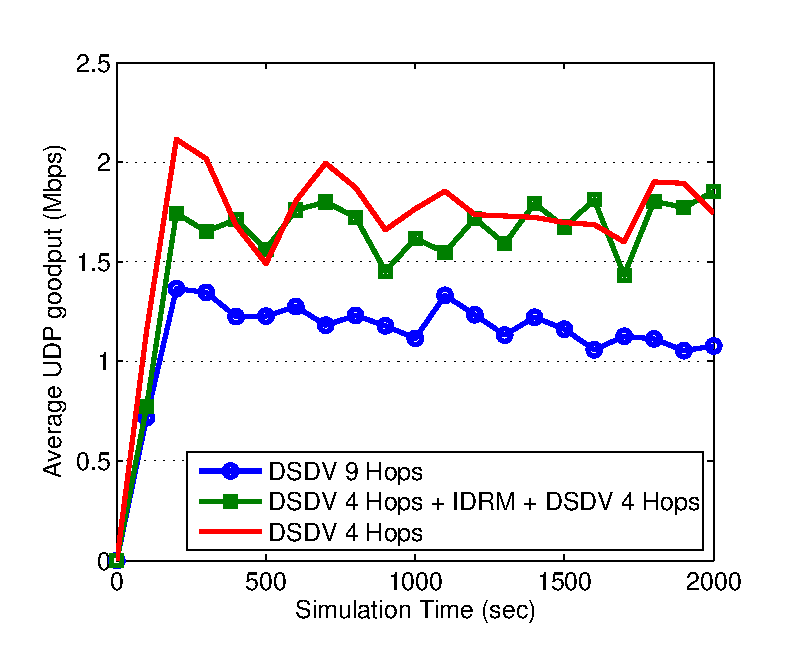
\includegraphics[width=0.47\textwidth, height=2.0in]{figs/case1DSDV.eps}
\caption{Aggregate UDP goodput for scenario 1}
\label{fig:case1udp}
\end{figure}

\begin{table}[htb!]
\center
\begin{tabular}{|c||c|c|c|c|}
\hline
 & IDRM & DSDV & Avgerage & Average\\
 & control pkts & control pkts & UDP goodput & E2E delay \\
\hline
DSDV 9 hops & N/A & 7353 & 1.115 Mbps &\\
\hline
DSDV 4 hops & N/A & 6891 & 1.547 Mbps &\\
\hline
IDRM + DSDV & 6309 & 5316 & 1.669 Mbps &\\
\hline
\end{tabular}
\caption{No. of control packets and average end-to-end delay}
\label{table:case1overhead}
\end{table}

The aggregate UDP goodput for all 3 cases are shown in figure \ref{fig:case1udp}.
IDRM with DSDV case performs better than DSDV 9 hops case because 
there are three independent channels, so the number of packet loss due to collision is less.

